\chapter{Hydrogeochemical Modelling}

Since the conceptual model is now set up, the idea can now be implemented inside PHREEQC.  In order to find the change in the chemical composition of the geothermal fluid due to the changes in the temperature and pressure, PHREEQC has been used extensively. 

It is important to mention that the modelling has been done without considering the gas phase and only saturation indices of carbonate minerals is considered. The minerals with their chemical formula are present in Table \ref{Minerals}: 


\begin{table}[h!]
\centering
\begin{tabular}{|l|l|}
\hline
\textbf{Mineral} & \textbf{Chemical Formula} \\ \hline
Aragonite        & CaCO$_3$                     \\ \hline
Calcite          & CaCO$_3$                     \\ \hline
Dolomite         & CaMg(CO$_3$)$_2$                \\ \hline
\end{tabular}
\end{table}
\label{Minerals}

Moreover, geothermal water selected for this batch simulation 
The idea behind checking the change in composition will be to look at the saturation index of the minerals. The saturation index is an index which can tell whether water will precipitate out as a particular mineral or will dissolve. The sign indicated whether the mineral is dissolved (if negative) or whether it is precipitated (if positive) or when water and mineral are in equilibrium (if zero) \cite{index."_2018}
\newline\newline

A change in temperature is only observed in the reinjection well, where the temperature can vary upto 150 degree celsius. As explained in the conceptual model, first the temperature of the fluid is maintained at 150 degree Celsius from the ground to the the re-injection well at a certain depth. There is a pressure drop from 500bar to about 200 bar. This is because of the fact that the well has less pressure than the ground. 
Once that is done, the same fluid composition is then carried out with an upward flow, where the temperature changes from 150 degree celsius to 25 degree celsius and pressure from 200 bar to 1 bar. A conceptual design is presented in \ref{fig:modelling_re}. However,these properties
of raw geothermal water can help in determining the intensity of the scaling phenomena which can exist on the surface of the nanofiltration membrane and can have an influence on total efficiency of the process. \cite{HILAL2004281}\cite{KAYA201510}
\newline
\newline

In the batch simulation process PHREEQC was used in order to simulate the mentioned conceptual model. The mentioned model is used with the help of using REACTION TEMPERATURE and REACTION PRESSURE were used extensively in order to work with the change in temperature and pressure. The chemical composition changes when it is cooled and when it is reinjected and hence the simulations are done at surface and reservoir temperature. 

It is important to mention about the composition of solution considered at 1 atm and 25 degree Celsius for a general solution present in The Netherlands. The data has been collected from a thesis done by another student at Delft University of Technology under supervision of Prof. Timo Heimovara at TU Delft.  \cite{van2012mineral} The geothermal water selected is set to be highly conductive with a very high hardness level by increasing the amount of calcium sulphates and magnesium. Some values which were found to be a bit absurd were taken from other resources and were then average in order to achieve a better result. \cite{tomaszewska2017assessment}
\begin{table}[h!]
\centering
\begin{tabular}{|l|l|}
\hline
\textbf{Sample} & \textbf{Concentration (Mg/kg)} \\ \hline
Ba              & 0.25                           \\ \hline
C               & 249.59                         \\ \hline
Ca              & 1350                           \\ \hline
Cl              & 4713 charge                    \\ \hline
K               & 74                             \\ \hline
Fe(2)           & 0.49                           \\ \hline
Li              & 2.44                           \\ \hline
Mg              & 18                             \\ \hline
Mn              & 1.28                           \\ \hline
Na              & 1670                           \\ \hline
S(6)            & 95.32                          \\ \hline
Sr              & 22                             \\ \hline
Zn              & 1.53                           \\ \hline
Si              & 1.3                            \\ \hline
\end{tabular}
\label{ChemComp}
\end{table}
\newline\newline
The idea behind solving this problem was to use first pure water in equilibrium with calcite and aragnoite in equilibrium with them. This was then by setting up an equilibrium using PHREEQC function EQUILIBRIUM PHASES as shown below: 
\newline
\newline
\begin{verbatim}
SOLUTION 1 Pure Water
	pH	7.0
	temp 	25.0
	EQUILIBRIUM_PHASES 
	Aragonite 0.0
	Calcite 0.0
    Dolomite    0.0
\end{verbatim}
\newline\newline
The solution was then mixed with the chemical composition mentioned in Table \ref{ChemComp} with a varieties of  ratio such as 7:3, 3:7, 5:5 where the first term is pure water and the second is chemical composition of the mentioned minerals in Table \ref{ChemComp} in order to change the phase of the composition. A phase with completely hard water solution has also been considered with only 1\% pure water. \cite{viveiros2015calcium}\cite{KAYA201510} This was achieved with the use of MIX function in PHREEQC where SOLUTION 1 which is pure water and SOLUTION 2 with the chemical composition. For example for a ratio of 7:3, this can be declared like:
\begin{verbatim}
    MIX 
    1   7.0
    2   3.0
\end{verbatim}

Finally the temperature and pressure were changed as mentioned in the conceptual model. This can also be seen from the Figure  \ref{fig:modelling_re} where the injection pressure is set at 300 bars considering that the reservoir pressure at 200 bars. This was achieved by using REACTION TEMPERATURE and REACTION PRESSURE functions of PHREEQC. For the injection well, the steps used are:
\begin{verbatim}
REACTION_TEMPERATURE 1
25 150 150 150 
REACTION_PRESSURE  1
1 300 300 200
\end{verbatim}

\newline
Using the same concept for production well, the changes were estimated as well, however REACTION TEMPERATURE was not considered due to the fact that there is no change in temperature observed:

\begin{verbatim}
    REACTION_PRESSURE 1
    200 100 100 1
\end{verbatim}


\begin{figure}[h!]
    \centering
    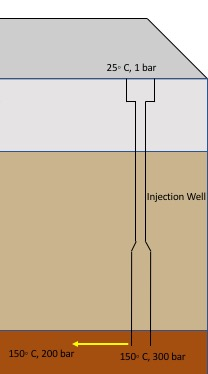
\includegraphics[scale=0.5]{mini-con.jpeg}
    \caption{Conceptual Design for Modelling input into PHREEQC for injection well}
    \label{fig:modelling_re}
\end{figure}

\newline 
As already mentioned earlier, PHREEQC didn't provide that good results for production well.  Due to the fact that most of the changes were in-situ conditions only, no scaling was found during the PHREEQC simulations, due to the fact that PHREEQC is sensitive on temperature and not on pressure this makes sense. 






